\documentclass{article}
\usepackage{fullpage}
\usepackage{graphicx}
\usepackage[aux]{rerunfilecheck}

\newcommand{\ds}{\displaystyle}

\title{MATH 110 Quiz 1 Solutions}
\author{Edward Doolittle}

\begin{document}
\maketitle
\begin{enumerate}
\item
  \begin{enumerate}
  \item The table is as follows.  The $9-x$ column is trivial,
    but you might want to double check with a calculator just in case.
    \begin{center}
      \begin{tabular}{|r|l|l|l|}
        \hline
	\rule{10pt}{0pt}$x$\rule{10pt}{0pt}     
	  & \rule{10pt}{0pt}$9-x$\rule{10pt}{0pt}
	  & \rule{10pt}{0pt}\rule{0pt}{12pt}$\sqrt{x}-3$\rule{10pt}{0pt}
	  & \rule{20pt}{0pt}$f(x)$\rule{20pt}{0pt} \\
	\hline
	\rule{0pt}{12pt}$10.00$ &   -1.0000    &+0.1623    &  -6.1623   \\
	\hline
	\rule{0pt}{12pt} $9.10$ &   -0.1000    &+0.01622   &  -6.0166   \\
	\hline
	\rule{0pt}{12pt} $9.01$ &   -0.01000   &+0.001666  &  -6.0017   \\
	\hline
	\rule{0pt}{12pt} $8.99$ &   +0.01000   &-0.001667  &  -5.9983   \\
	\hline
	\rule{0pt}{12pt} $8.90$ &   +0.1000    &-0.01671   &  -5.9833   \\
	\hline
	\rule{0pt}{12pt} $8.00$ &   +1.0000    &-0.1716    &  -5.8284   \\
	\hline
      \end{tabular}
    \end{center}
    Note that to have four decimal points of accuracy in the final column,
    I had to keep more than four decimal points in the intermediate 
    calculations; I had to keep four significant figures (five would have
    been better).
  \item % 1(b)
    Based on the above table, a reasonable guess for the limit would be
    a number about halfway between $-6.0017$ and $-5.9983$, i.e., about
    $-6.0000$ to four decimal places.  (Using limit theorems, we can now
    show that that is the exact answer.)
  \end{enumerate}
\item % 2
  Candidates for vertical asymptotes of rational functions 
  are vertical lines over $x$ values at which the denominator goes to $0$.
  The denominator goes to $0$ when $x-3=0$, so
  our candidates for an asymptote is the line $x=3$.  The
  rational function may have a removable discontinuity at that $x$ value
  rather than an infinite discontinuity, however, so we must check (one-sided)
  limits as $x$ approaches that candidate value.  
  %Note that
  %\begin{equation*}
  %  \lim_{x\to a} \frac{x+3}{(x+3)(x-2)} = \lim_{x\to a} \frac{1}{x-2}$
  %\end{equation*}
  %for any $a$, so we can use the latter simpler function in our calculations.

  For $\ds \lim_{x\to 3^-}$ we have $x-3$ slightly smaller than $0$ and
  the denominator $(x+3)(x-2)$ close to $6\times 1$ which is positive,
  so $\ds \lim_{x\to 3^-} \frac{(x+3)(x-2)}{x-3}$ is $-\infty$.

  For $\ds \lim_{x\to 3^+}$, again the numerator is close to $6$, a positive
  number, and the denominator tends to $0$ from above, so is positive and small,
  so the limit
  $\ds \lim_{x\to 3^+} \frac{(x+3)(x-2)}{x-3}$ is $+\infty$.

  In summary, there is one and only one vertical asymptote, at $x=3$.  
  %See the graph
  %in Figure~\ref{fig:graph-hole-asymptote}.
  %\begin{figure}
  %  \begin{center}
  %    \includegraphics{graph-(x+3)div(x+3)(x-2).eps}
  %  \end{center}
  %  \caption{Graph of $\ds y=\frac{x+3}{x^2+x-6}$}
  %  \label{fig:graph-hole-asymptote}
  %\end{figure}
  %Note that there is a hole in the graph at $x=-3$ but no asymptote there.
\end{enumerate}

\end{document}


\begin{enumerate}
\item 
  \begin{enumerate}
  \item Let\marginpar{\centering (10)}
    $\ds f(x)=\frac{4-\sqrt{x}}{x-16}$.
    Use your calculator to 
    fill in the following table of values to 4 decimal points.
    \begin{center}
      \begin{tabular}{|l|l|l|l|}
        \hline
	\rule{10pt}{0pt}$x$\rule{10pt}{0pt}     
	  & \rule{10pt}{0pt}\rule{0pt}{12pt}$4-\sqrt{x}$\rule{10pt}{0pt}
	  & \rule{10pt}{0pt}$x-16$\rule{10pt}{0pt}
	  & \rule{20pt}{0pt}$f(x)$\rule{20pt}{0pt} \\
	\hline
	\rule{0pt}{12pt}$17.00$ &              &        &        \\
	\hline
	\rule{0pt}{12pt}$16.10$ &              &        &        \\
	\hline
	\rule{0pt}{12pt}$16.01$ &              &        &        \\
	\hline
	\rule{0pt}{12pt}$15.99$ &              &        &        \\
	\hline
	\rule{0pt}{12pt}$15.90$ &              &        &        \\
	\hline
	\rule{0pt}{12pt}$15.00$ &              &        &        \\
	\hline
      \end{tabular}
    \end{center}
  \item Use the table of values to estimate the limit
    $\displaystyle\lim_{x\to 16} \frac{4-\sqrt{x}}{x-16}$.
  \end{enumerate}
\newpage
\item Find\marginpar{\centering (10)} the vertical asymptotes of the function
  $\displaystyle y = \frac{x+1}{x^2+x-6}$.
\end{enumerate}

\end{document}

